\subsection*{Problema 07}

\textbf{Enunciado:} Calcular la integral:
\begin{equation*}
  \int \frac{dx}{\sqrt{4x^2 + 4x - 3}}
\end{equation*}

\textbf{Solución:} 

Comenzamos completando el cuadrado 
dentro de la expresión radical del 
denominador. Tomamos la expresión 
cuadrática:
\begin{align*}
  4x^2 + 4x - 3 &= 4(x^2 + x) - 3 \\
  &= 4\left(x^2 + x + \frac{1}{4} - \frac{1}{4}\right) - 3 \\
  &= 4\left(x + \frac{1}{2}\right)^2 - 1 - 3 \\
  &= 4\left(x + \frac{1}{2}\right)^2 - 4
\end{align*}

También podemos escribirlo como:
\begin{equation*}
  4x^2 + 4x - 3 = (2x + 1)^2 - 4
\end{equation*}

Sustituyendo esto en la integral 
original, obtenemos:
\begin{align*}
  I &= \int \frac{dx}{\sqrt{(2x + 1)^2 - 4}}
\end{align*}

Utilizamos la sustitución 
trigonométrica secante. 
Hacemos el cambio de variable:
\begin{equation*}
  2x + 1 = 2\sec\theta
\end{equation*}

Derivando ambos lados para 
encontrar el diferencial $dx$:
\begin{align*}
  2\,dx &= 2\sec\theta\tan\theta\,d\theta \\
  dx &= \sec\theta\tan\theta\,d\theta
\end{align*}

Sustituimos $2x + 1$ y $dx$ 
en la integral:
\begin{align*}
  I &= \int \frac{\sec\theta\tan\theta\,d\theta}{\sqrt{(2\sec\theta)^2 - 4}} \\
  &= \int \frac{\sec\theta\tan\theta\,d\theta}{\sqrt{4(\sec^2\theta - 1)}}
\end{align*}

Empleamos la identidad trigonométrica 
fundamental $\sec^2\theta - 1 = \tan^2\theta$:
\begin{align*}
  I &= \int \frac{\sec\theta\tan\theta\,d\theta}{\sqrt{4\tan^2\theta}} \\
  &= \int \frac{\sec\theta\tan\theta\,d\theta}{2\tan\theta} \\
  &= \frac{1}{2}\int \sec\theta\,d\theta
\end{align*}

La integral de la secante es un 
resultado estándar conocido:
\begin{equation*}
  I = \frac{1}{2}\ln\left|\sec\theta + \tan\theta\right| + C
\end{equation*}

A partir de la sustitución original 
$2x + 1 = 2\sec\theta$, despejamos 
la secante:
\begin{equation*}
  \sec\theta = \frac{2x + 1}{2}
\end{equation*}

Para encontrar $\tan\theta$, 
utilizamos la identidad 
$\tan\theta = \sqrt{\sec^2\theta - 1}$:
\begin{align*}
  \tan\theta &= \sqrt{\left(\frac{2x + 1}{2}\right)^2 - 1} \\
  &= \sqrt{\frac{4x^2 + 4x + 1 - 4}{4}} \\
  &= \frac{\sqrt{4x^2 + 4x - 3}}{2}
\end{align*}

Sustituimos las expresiones 
de $\sec\theta$ y $\tan\theta$ 
en términos de $x$:
\begin{align*}
  I &= \frac{1}{2}\ln\left|
  \frac{2x + 1}{2} + \frac{\sqrt{4x^2 + 4x - 3}}{2}
  \right| + C
\end{align*}

Aplicando propiedades de los 
logaritmos para simplificar 
la constante del denominador:
\begin{align*}
  I &= \frac{1}{2}\ln\left|
  2x + 1 + \sqrt{4x^2 + 4x - 3}
  \right| \\
  &\quad - \frac{1}{2}\ln(2) + C
\end{align*}

Agrupando la constante $-\frac{1}{2}\ln(2)$ 
con la constante de integración $C$, 
obtenemos la solución general final:
\begin{align*}
  I &= \frac{1}{2}\ln\left|
  2x + 1 + \sqrt{4x^2 + 4x - 3}
  \right| + C
\end{align*}

\begin{figure}[H]
	\centering
	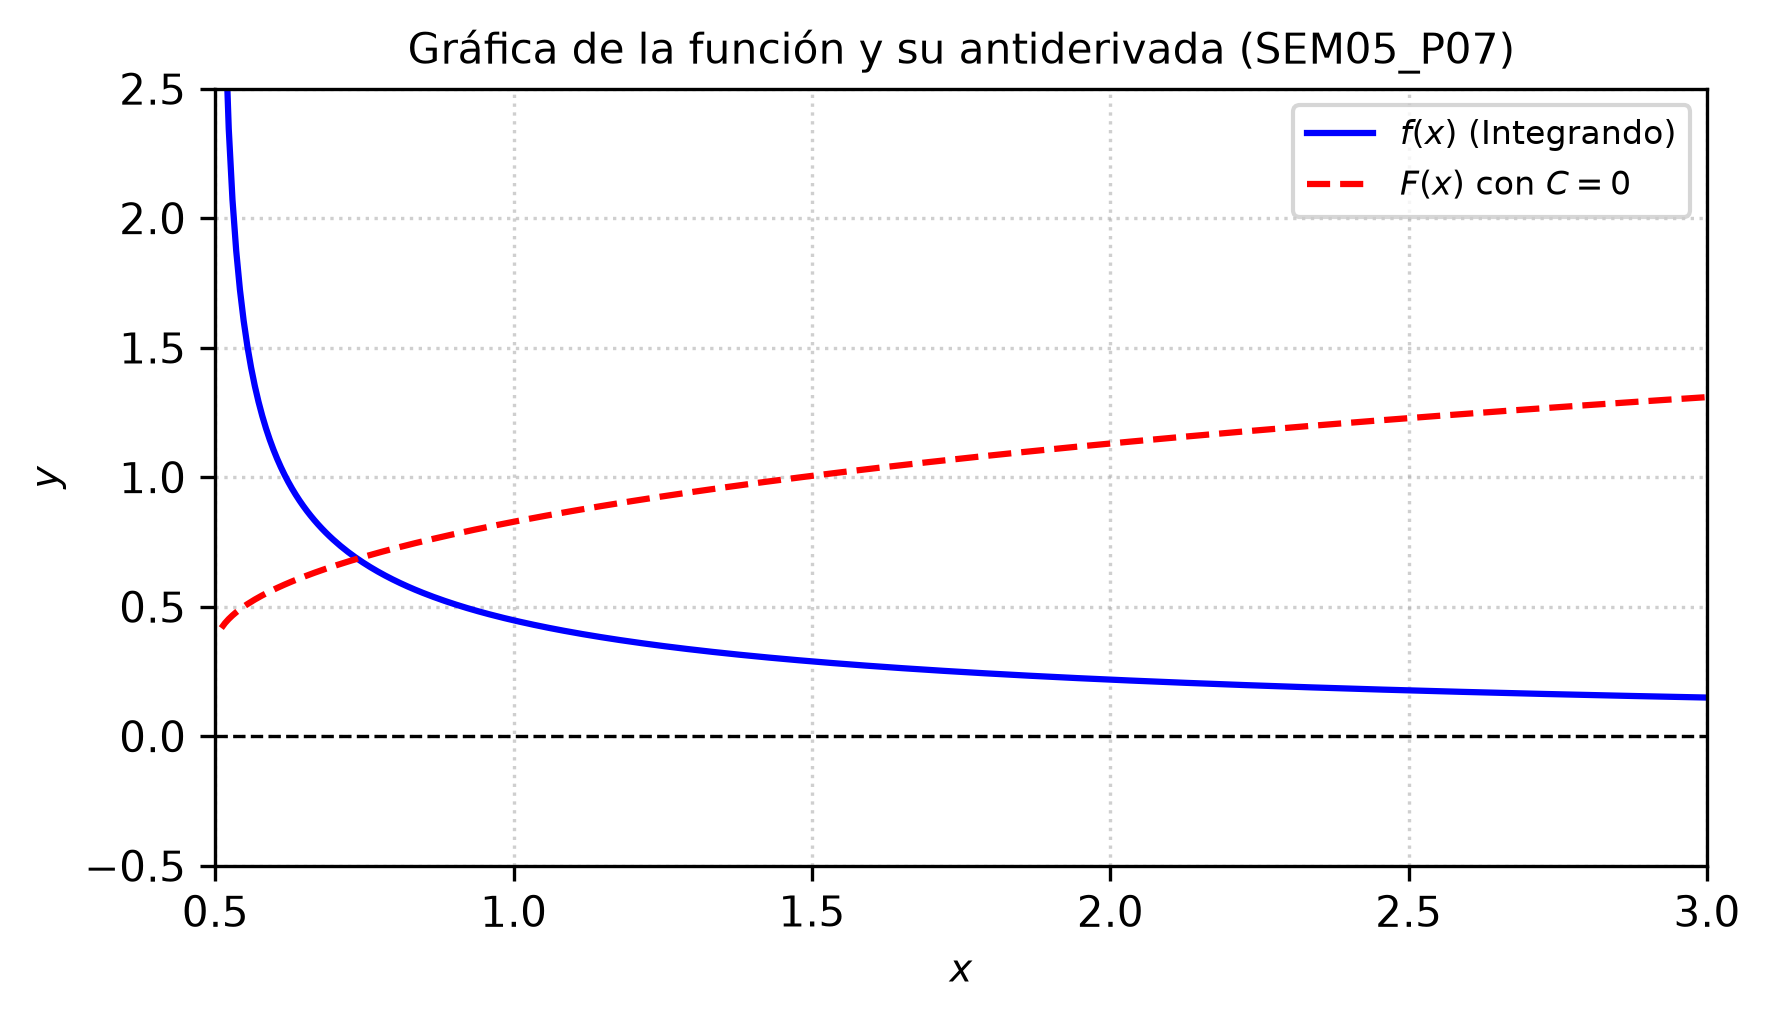
\includegraphics[width=\columnwidth]{semana_05/graficas/SEM05_P07_grafica.png}
	\caption{Representación gráfica de $f(x)$ y su antiderivada $F(x)$ evaluada para la constante de integración $C = 0$ (Problema 07).}
	\label{fig:problema07}
\end{figure}
